%==========================================================================

\begin{frame}[fragile]

  {\Huge General Enhancements}

  \vspace{10pt}

\end{frame}

%==========================================================================

% Examples

% note: always keep the [fragile] for your frames!

%\begin{frame}[fragile]{Example list}
%  \begin{itemize}
%      \item Item 1
%      \item Item 2 with some \texttt{code}
%      \begin{itemize}
%        \item Sub-item 2.1
%        \item Sub-item 2.2
%      \end{itemize}
%  \end{itemize}
%\end{frame}

%\begin{frame}[fragile]{Example code}
%    \begin{code}[keywords={std}]
%        #include <iostream>
%
%        int main() {
%            std::cout << "hello world\n";
%        }
%    \end{code}
%\end{frame}

%\begin{frame}[fragile]{Example table}
%    \begin{center}
%        \begin{tabular}{l|l}
%            a & b \\\hline
%            c & d
%        \end{tabular}
%    \end{center}
%\end{frame}

%==========================================================================

\begin{frame}[fragile]{MDRange}
  \begin{itemize}
    \item Improvements on the MDRange internals on device when the iteration domain is small enough
  \end{itemize}
  \begin{center}
    
\includegraphics[width=0.5\textwidth]{no_grid_stride_loop.png}
  \end{center}
\end{frame}

%==========================================================================

\begin{frame}[fragile]{SIMD}
  \begin{itemize}
    \item Add \texttt{std::uint32\_t} support for NEON
    \item Improve the performance of generator constructors on SVE
    \item Make the flag argument for memory operations optional
    \begin{code}[breakatwhitespace=true,breaklines=true,language=C++]
Experimental::simd<T> vec(ptr, Experimental::simd_flag_default);
Experimental::simd_unchecked_store(vec, ptr, Experimental::simd_flag_default);
    \end{code} \\
      Becomes:
    \begin{code}[language=C++]
Experimental::simd<T> vec(ptr);
Experimental::simd_unchecked_store(vec, ptr);
    \end{code}
  \end{itemize}
\end{frame}

%==========================================================================

\begin{frame}[fragile]{Graph}
  \begin{itemize}
    \item Rename \texttt{native\_graph()} and \texttt{native\_graph\_exec()} to backend specific names \texttt{\{cuda,hip,sycl\}\_graph()} and \texttt{\{cuda,hip,sycl\}\_graph\_exec()}
    \item Add a \texttt{GraphNodeKind} enum and allow to retrieve the node type
    \begin{itemize}
      \item at compile time: \texttt{NodeType::node\_kind}
      \item at runtime: \texttt{node.get\_node\_kind()}
    \end{itemize}
    \item Allow access to vendor nodes with \texttt{node.\{cuda,hip,sycl\}\_node()}
  \end{itemize}
\end{frame}

%==========================================================================

\begin{frame}[fragile]{Atomics}
   Improve performance of load/store atomic by leveraging compiler built-ins instead of generating them via CAS
  \begin{figure}[!htb]
     \centering
     \begin{minipage}{0.325\textwidth}
       \centering
       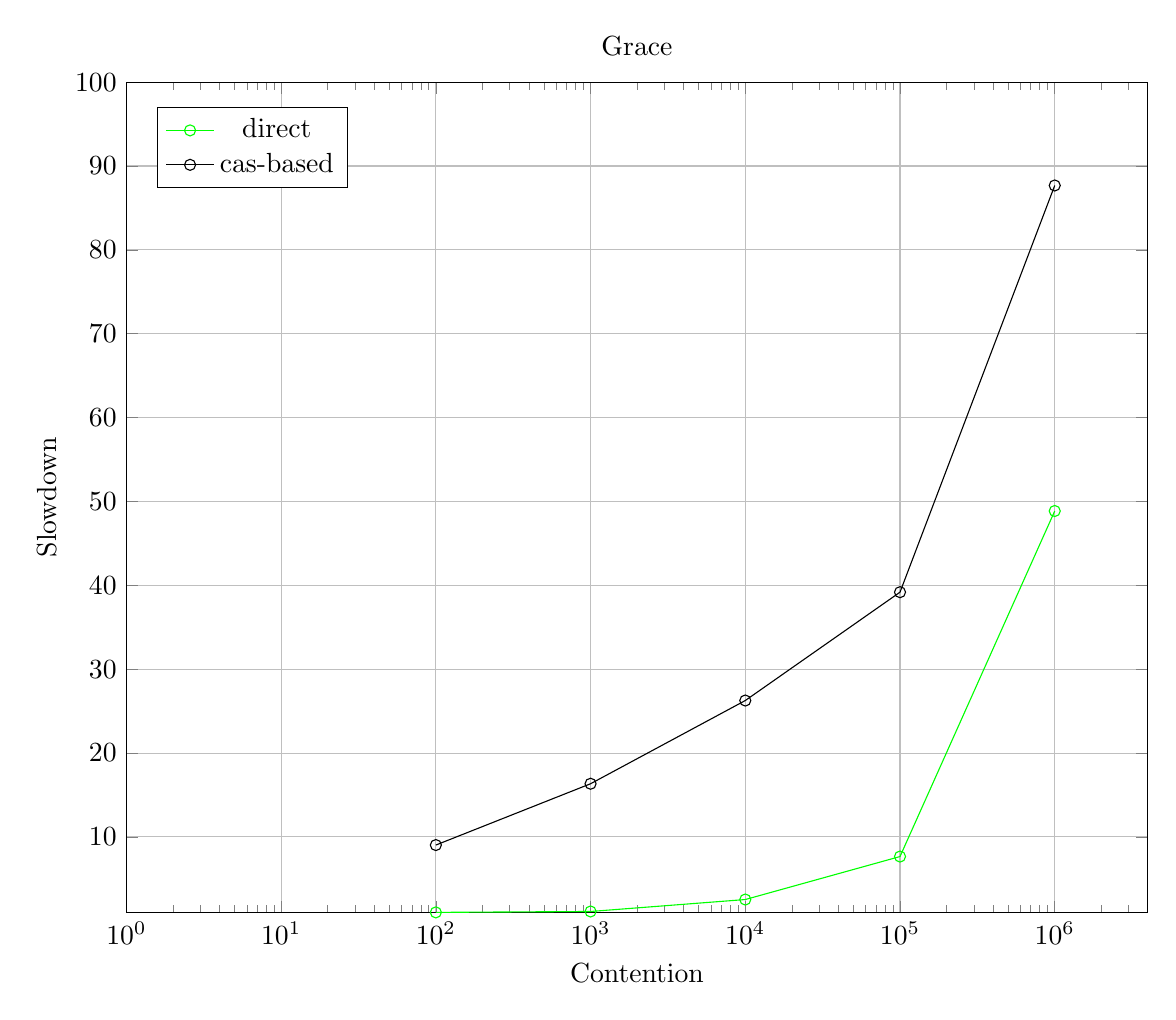
\begin{tikzpicture}
         \begin{semilogxaxis}[
             title={Grace},
         width=1.2\textwidth,
         height=1.0\textwidth,
         log basis x = 10,
         grid=major,
         xmin=1,
         xlabel={Contention},
         ylabel={Slowdown},
         ymin=1,
         ymax=100,
         legend pos=north west
         ]
         %cpu
         \addplot+[mark=o, color=green] coordinates {
         (100,1.0)
         (1000,1.1088313941)
         (10000,2.5329092838)
         (100000,7.6595455536)
         (1000000,48.8640858911)
          };
         %cpu
         \addplot+[mark=o, color=black] coordinates {
         (100,9.02886777711)
         (1000,16.3405593973)
         (10000,26.2635370966)
         (100000,39.1844956122)
         (1000000,87.6812757724)
             };
         \legend{direct,cas-based}
         \end{semilogxaxis}
       \end{tikzpicture}
     \end{minipage}
     \hspace{1cm}
     \begin{minipage}{0.325\textwidth}
       \centering
       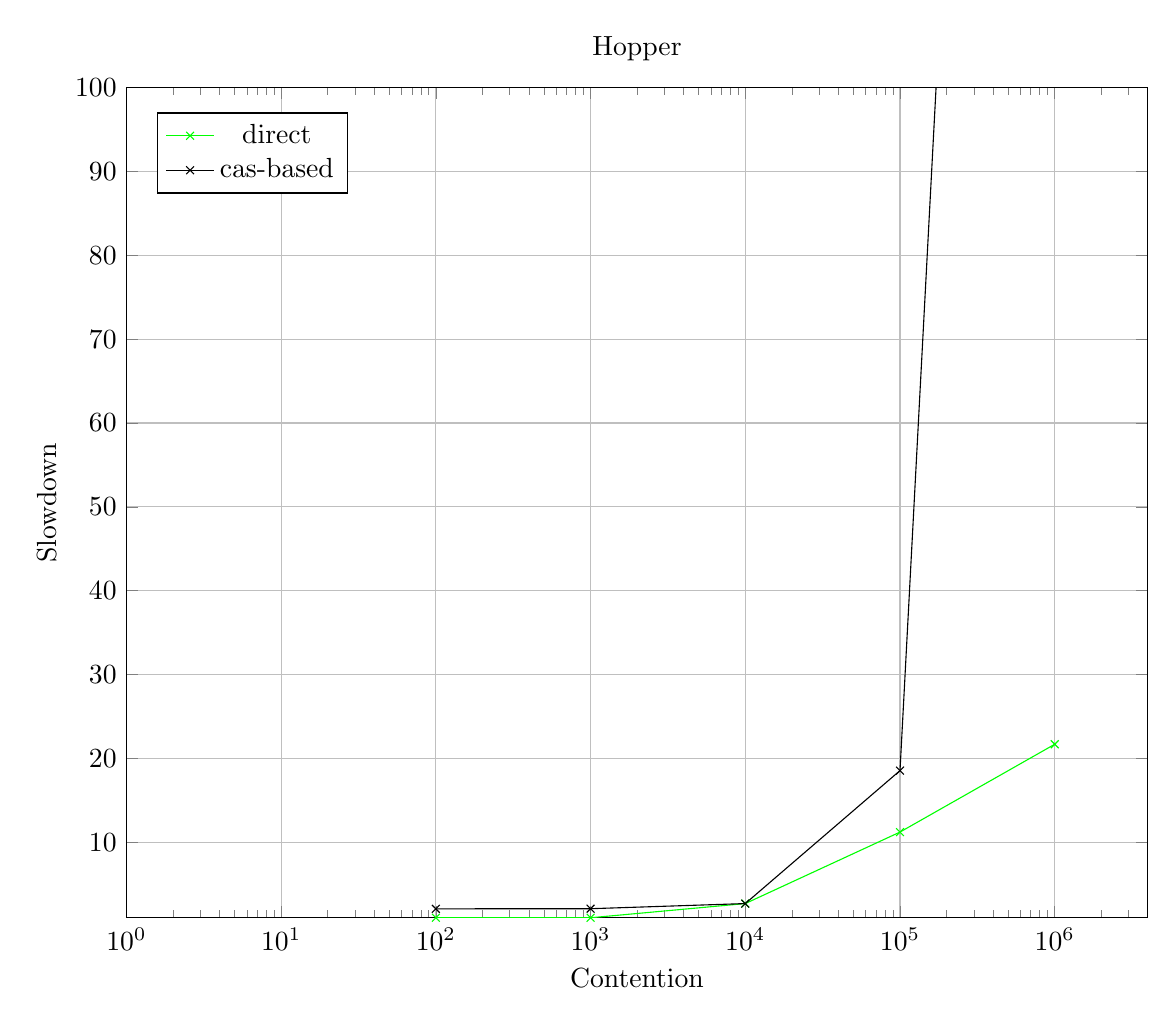
\begin{tikzpicture}
         \begin{semilogxaxis}[
             title={Hopper},
         width=1.2\textwidth,
         height=1.0\textwidth,
         log basis x = 10,
         grid=major,
         xmin=1,
         xlabel={Contention},
         ylabel={Slowdown},
         ymin=1,
         ymax=100,
         legend pos=north west
         ]
         %grace-hopper 200 reference on on-cas
         %non-cas
         %gpu
         \addplot+[mark=x, color=green] coordinates {
         (100,1.0)
         (1000,1.0)
         (10000,2.6924211572)
         (100000,11.2185832364)
         (1000000,21.6895538258)
             };
          % cas-based
          %gpu
          \addplot+[mark=x, color=black] coordinates {
         (100,2.06410845404)
         (1000,2.08026722305)
         (10000,2.6912696104)
         (100000,18.5523211491)
         (1000000,368.08750952935)
             };
         \legend{direct,cas-based}
         \end{semilogxaxis}
       \end{tikzpicture}
     \end{minipage}%
     \caption{1e9 \texttt{atomic\_load/store} operations on \texttt{int} with various contention}
  \end{figure}
\end{frame}

%==========================================================================
\begin{frame}[fragile]{Miscellaneous (1/2)}
  \begin{itemize}
    \item Introduce \texttt{KOKKOS\_FORCEINLINE\_[CLASS\_]LAMBDA} macros
    \item Support \texttt{FORCEINLINE} macros with MSVC
    \item Support building and using Kokkos libraries as C++ modules with MSVC and GCC 16
    \item Throw a new \texttt{Experimental::BadAlloc} exception on allocation failures
    \item Increase the maximum level 1 scratch size from 20MB to 80MB
  \end{itemize}
\end{frame}

%==========================================================================

\begin{frame}[fragile]{Miscellaneous (2/2)}
  \begin{itemize}
    \item Make execution space's move constructor and assignment operator \texttt{noexcept}
    \item Make \texttt{View}'s move constructor \texttt{noexcept}
    \item Add signed \texttt{index\_type} and unsigned \texttt{size\_type} aliases to execution and memory spaces
    \item Promote numeric traits out of the \texttt{Experimental::} namespace into \texttt{Kokkos::}
    \item Use the mathematical constants from the standard library
  \end{itemize}
\end{frame}

%==========================================================================

\begin{frame}[fragile]{StdAlgorithms}
  \begin{itemize}
    \item Extract iterator related functions from \texttt{algorithms} to \texttt{core}
      \begin{itemize}
        \item \texttt{Kokkos::Experimental::begin}
        \item \texttt{Kokkos::Experimental::end}
        \item \texttt{Kokkos::Experimental::cbegin}
        \item \texttt{Kokkos::Experimental::cend}
        \item \texttt{Kokkos::Experimental::distance}
      \end{itemize}
    \item Check preconditions on view extents in the algorithms
  \end{itemize}
\end{frame}
